\chapter[Modellierung als Computerprogramm]{Modellierung von Patchwork als Computerprogramm}
\label{chapter:modellierung-von-patchwork-als-computerprogramm}

Ein wesentlicher Schritt in der Entwicklung von Computerspielengines besteht in der Modellierung und Umsetzung des Spiels als Computerprogramm. Da Engines in der Regel darauf basieren mehrere zehntausende von Aktionen vorrausschauen \cite{2018.AlphaZero}, muss die zugrundeliegende Implementierung so effizient wie möglich sein. Eine erste prototypische Implementierung von Patchwork in Python führte zu Zuggenerierungszeiten von ca. $100\acs{ms}$, was in 10 Sekunden aber gerade mal die Analyse von 100 möglichen Zügen bedeutet. Aus diesem Grund wird Patchwork mit der Programmiersprache \emph{Rust} \cite{2014.Rust} umgesetzt. Rust hat Performance als ein Hauptziel und zeichnet sich durch eine schnelle und speichereffiziente Ausführung aus \cite{2024.Rust}. Zusammen mit weiteren Effizienzoptimierungen führt dies zu Ausführungszeiten im Mirkosekundenbereich (Tabelle \ref{tabelle:patchwork-methods}).

\lstinputlisting[
    label={code:patchwork-state},
    caption={Patchwork-Zustand},
    captionpos=b,
    language=Rust,
    firstline=0,
]{res/code/patchwork-state.rs}

Der gesamte Zustand von Patchwork wird zu jeder Zeit durch die in Codeausschnitt \ref{code:patchwork-state} dargestellte Struktur \code{Patchwork} repräsentiert. Alle noch verfügbaren Flicken werden in \code{patches} in der Reihenfolge gespeichert, wie sie vor der Spielfigur liegen. Der \code{turn\_type} zeigt an, ob es sich bei den derzeit verfügbaren Aktionen um eine normale Aktion handelt oder ob ein Spezialflicken gelegt werden muss. Der derzeitige Spieler, der Inhaber des $7\times 7$ Sonderplättchens und der Spieler, welcher als erstes das Ziel erreicht hat, werden im Bitfeld \code{status\_flags} festgehalten, sofern vorhanden. Letzteres ist relevant, um bei einem beendeten Spiel mit gleicher Punktzahl den Gewinner identifizieren zu können.

Der Zeitplan wird mittels der \code{TimeBoard}-Struktur modelliert. Diese hält intern nur ein einfache \ac{u8}-Array der Länge 54. Bei jedem Eintrag des Arrays handelt es sich wiederrum um ein Bitfeld. Dieses kann signalisieren, ob sich Spieler 1 und 2, ein Knopfeinkommen oder ein Spezialflicken auf ihrem Feld befindet. Knopfeinkommen und Spezialflicken befinden sich im originalen Spiel zwischen 2 Feldern. Im Array werden sie einfach in dem Feld nach ihrer Originalposition gespeichert. Sobald solch ein Feld von einem Spieler erreich wird, tritt der Effekt ein, was zu gleichem Verhalten wie im Brettspiel führt.

Zuletzt existiert für jeden Spieler noch ein Zustand in der Patchwork-Struktur. Der Zustand jeden Spielers setzt sich dabei aus 3 Komponenten zusammen. Zuerst wird hier auch die Position des Spielers gespeichert, um Zugriff in konstanter Zeit zu ermöglichen. Weiterhin wird der derzeitig verfügbare Knopfvorrat des Spielers gespeichert. Zuletzt wird noch auf eine weitere Struktur, das \code{QuiltBoard}, verwiesen.

\section{Aufbau des Ablageplans}

\lstinputlisting[
    label={code:quilt-board-definition},
    caption={Definition der QuiltBoard-Struktur},
    captionpos=b,
    language=Rust,
    firstline=0,
]{res/code/quilt-board-definition.rs}
\vspace*{-0.3cm}

Die in Codeausschnitt \ref{code:quilt-board-definition} definierte Struktur \code{QuiltBoard} modelliert den Ablageplan eines Spielers. Dabei existieren nur 2 Attribute. Zuerst wird das Knopfeinkommen mit \code{button\_income} gespeichert, was durch die auf dem Ablageplan liegenden Flicken beim Passieren einer Knopf-Wertung generiert wird. Das zweite Attribut \code{tiles} dient dazu, den Status der einzelnen Felder auf dem Ablageplan zu speichern. Der Ablageplan besteht aus 81 Feldern, die in 9 Zeilen und 9 Spalten angeordnet sind, und für die jeweils gespeichert werden muss, ob das Feld belegt ist oder nicht. Da alle Abfragen bezüglich Status der Felder so schnell wie möglich sein sollen, kommt hier anstatt eines üblichen 2-dimensionalen Arrays eine \ac{u128} zum Einsatz. Da nur zwei Zustände existieren, kann für jedes Feld ein Bit verwendet werden. Weiterhin werden alle Felder des Ablageplans zeilenweise wie in Abbildung \ref{fig:quilt-board-storage} in einer Ganzzahl nacheinander abgelegt.

\vspace*{-5cm}
\pagebreak

\begin{figure}[!ht]
    \centering
    \rlap{{\color{white}\acf{LSB} \acf{MSB}}} \vspace*{-\baselineskip}
    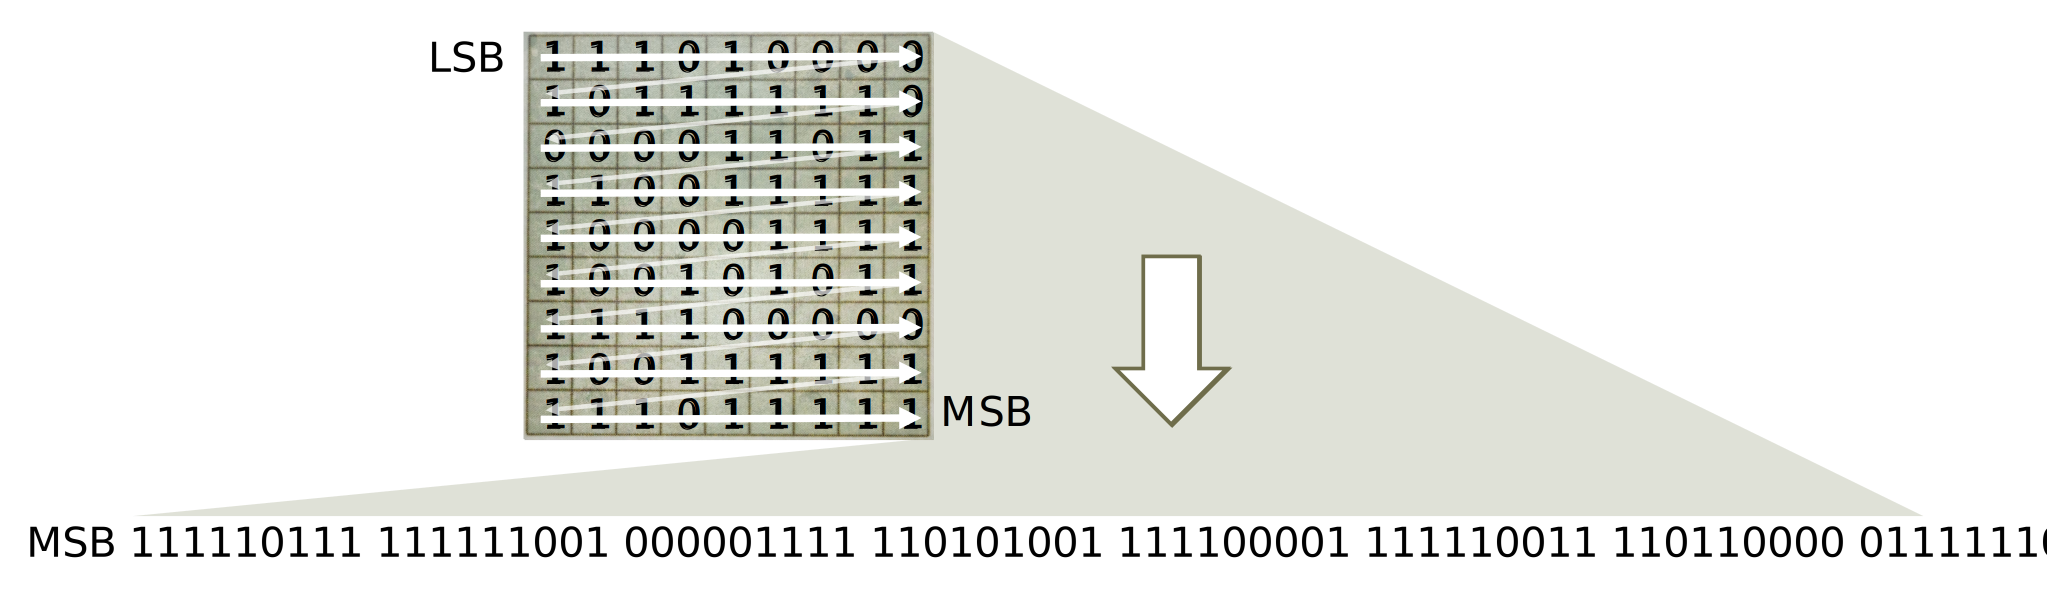
\includegraphics[width=\textwidth]{res/pictures/quilt-board-storage.pdf}
    \caption{Zeilenweise Anordnung der Felder des Ablageplans}
    \label{fig:quilt-board-storage}
\end{figure}

Da der Ablageplan 81 Felder umfasst, muss $2^7=128$ Bit als Ganzzahldatentyp verwendet werden. Dieser wird von Rust nativ unterstützt und für 64 Bit Rechner in mehrere Operationen kompiliert. Die oberen Bits der Zahl sind dabei immer auf 0 gesetzt. Durch die effiziente Speicherung des Ablageplans in einem \ac{u128}, können Abfragen bezüglich Befüllung oder Überlagerung von Feldern in konstanter Zeit durch Bitmasken und Bitoperationen durchgeführt werden. Als Beispiel lässt sich hier die Methode zum Überprüfen der notwendigen Bedingung zur Erhaltung des $7\times 7$ Sonderplättchen anführen (Anhang \ref{code:quilt-board-special-tile-condition}).

Besonders anzumerken ist, dass die Flicken und ihre Transformationen, wie sie auf dem Ablageplan liegen, nicht gespeichert werden. Da einige Computergegner wie beispielsweise der \ac{MCTS}-Spieler den Spielstand sehr oft kopieren müssen und die genaue Position der Flicken für die Generierung und Ausführung von Aktionen nicht benötigt wird, würde diese Extrainformation nur zu unnötig erhöhtem Speicherverbrauch führen.

\section{Modellierung der Aktionen}

Wie in Codeauschnitt \ref{code:action} zu sehen, sind die Spielzüge von Patchwork für das Computerspiel als \code{enum} umgesetzt, das folgende Aktionen definiert:
\begin{itemize}
    \item Die Aktion \code{Walking} beschreibt die Laufaktion eines Spielers startend vom Feld \code{starting\_index}.
    \item Die Aktion \code{PatchPlacement} beschriebt das Platzieren des Flickens mit der einzigartigen \ac{ID} \code{patch\_id}. Der Flicken muss einer der drei durch den aktuellen Spieler auswählbaren Flicken sein und wird unter diesen mit dem \code{patch\_index} identifiziert. In \code{patch\_transformation\_index} wird die jegliche Transformation des Flickens gespeichert, d.h. wie der Flicken gespiegelt, rotiert und wo er auf dem Spielfeld abgelegt wurde. Ob im vorigen Zug Spieler 1 an der Reihe war, wird im Attribut \code{previous\_player\_was\_1} gespeichert.
    \item Bei der Aktion \code{SpecialPatchPlacement} wird ein Spezialflicken auf das Spielfeld auf die Position des \code{quilt\_board\_index} gelegt.
    \item Die Aktion \code{Phantom} beschriebt einen Spielzug, indem der Spieler nichts tut. Diese Aktion kann im normalen Spielverlauf nicht vorkommen, wird allerdings für einige \ac{KI}-Gegner benötigt. Dies ist der Fall, in dem ein erzwungener Spielerwechsel stattfinden soll, also für die Situation in der eigentlich Spieler 1 an der Reihe wäre, aber Spieler 2 jetzt ziehen soll.
    \item Die Aktion \code{Null} kennzeichnet einen illegalen Zug.
\end{itemize}

\lstinputlisting[
    label={code:action},
    caption={Definition des Tagged-Union \code{Action}},
    captionpos=b,
    language=Rust,
    firstline=0,
]{res/code/action.rs}

Um diese Aktionen kompakter zu speichern und die effizientere Verarbeitung mit einem Computer zu ermöglichen, existiert die Struktur \code{ActionId}, welche aus einer Variablen mit dem Typ \ac{u32} besteht. In dieser einen Zahl der folgenden Ganzzahl-Intervalle werden alle Aktionen als Surrogat eindeutig codiert und wie folgt gespeichert:
\begin{itemize}
    \item Eine \ac{ID} aus $[0, 52]$ beschreibt die Laufaktion, wobei die Zahl das Startfeld repräsentiert.
    \item Eine \ac{ID} aus $[53, 133]$ beschreibt den Ablageort eines Spezialflickens, die Zahl repräsentiert die Position mittels Spielfeldindex.
    \item Eine \ac{ID} aus $[134, 88.837]$ beschreibt eine Flickenplatzierung, wobei dieselben Information wie bei dem vorher beschriebenen \code{Action}-Enum codiert gespeichert werden.
    \item Die Zahl 88.838 repräsentiert die Phantom-Aktion und folgende Zahl 88.839 die Null-Aktion.
\end{itemize}
Während die \code{ActionId} sehr gut für die Spielimplementierung geeignet ist, eignet sich diese aber nicht für die Ausgabe eines neuronalen Netzes. Ein Computernetzwerk sollte immer entscheiden, welche der ersten drei Flicken platziert werden soll. Die \code{ActionId} besitzt für diese Aufgabe durch ihren großen Zahlenbereich von ca. 90.000 Werten zu viel Overhead. So werden unter anderem für die Entscheidung unnötige Informationen wie der genaue Transformationsindex in der \code{ActionId} gespeichert. Aus diesem Grund existiert noch die \code{NaturalActionId}, welche als \ac{u64} Zahl kodiert ist. Hierbei wird mit der \ac{ID} 0 die Laufaktion codiert. Von 1 bis 81 werden die Platzierung für Spezialflicken mit Zeilen- und Spalteninformation codiert. Im Gegensatz zur \code{ActionId} werden danach alle weiteren Aktionen, die Flickenplatzierungen, im Bereich von 82 bis 2.025 codiert, indem nur gespeichert wird, welcher der ersten drei Flicken gewählt wurde und in welcher Reihe, Spalte, Rotation und Orientierung der Flicken platziert wurde. Die letzten beiden Zahlen codieren wieder die Phantom-Aktion (2.026) und die Null-Aktion (2.027).

Die oberen Bits der \code {NaturalActionId} werden zur Speicherung von Informationen verwendet, welche für die Umwandlung zurück in eine \code{ActionId} benötigt werden. Für die Ausgabe eines neuronalen Netzes sind diese Bits nicht relevant.

\section{Flicken}

Die Speicherung der Flicken im Computerprogramm ist aufwendiger. Der \code{PatchManager} übernimmt die Verwaltung der Flicken und stellt eine zentrale Zugriffmöglichkeit auf alle Flicken in der gesamten Applikation dar. So kann über den PatchManager beispielsweise die zufällige initiale Flickenreihenfolge zum Spielstart generiert werden oder ein Index auf dem Zeitplan zu einem konkretem Spezialflicken bidirektional zugeordnet werden. Um sicherzustellen, dass es immer nur genau eine Instanz des PatchManagers existiert, wird dabei das Entwurfsmuster Singleton implementiert \cite[S. 127]{2000.Gamma}.

Ein Flicken wird im Code als Patch bezeichnet und besteht aus einem eindeutigen Identifizierter, Knopf- und Zeitkosten sowie Knopfeinkommen. Der PatchManager speichert alle Patches in einem Array und erlaubt den Zugriff auf diese. Neben diesen einfachen Patch-Strukturen erlaubt der PatchManager aber auch noch Zugriff auf die sogenannten PatchTransformationen für jeden Flicken. Da der Ablageplan als eine einzige 81-bit lange Zahl abgespeichert ist, sind das Erkennen von Überlappungen und das Legen von Flicken in konstanter Zeit durch Und- sowie Oder-Bitoperationen möglich. Dafür muss nur für jeden Flicken und jede Platzierungsmöglichkeit die passende Zahl nach der gleichen Anordnung wie beim Ablageplan generiert werden. Die Erzeugung solch einer Zahl zur Laufzeit dauert jedoch im Vergleich zu anderen Operationen viel zu lange. Da die Anzahl der Flicken und ihrer Platzierungsmöglichkeiten aber begrenzt sind, kann für jeden Flicken bereits jede Mögliche Platzierungslage als \ac{u128} vorausberechnet werden. Der PatchManager hält dann alle diese vorausberechneten Transformationen in einer Liste. Eine Transformation besteht dabei neben der vorausberechneten Zahl noch aus dem genauen Platzierungsort mit Zeile, Spalte und der Transformation (Drehung sowie Spiegelung). Zuletzt speichert der PatchManager noch die genauen Felder der Flicken als $m\times n$-Matrix zu Darstellungszwecken. Alle drei Datentypen sind auch in Codeauschnitt \ref{code:patch} dargestellt.

\lstinputlisting[
    label={code:patch},
    caption={\code{PatchManager}, \code{Patch} und \code{PatchTransformation}},
    captionpos=b,
    language=Rust,
    escapeinside={<*}{*>},
    firstline=0,
]{res/code/patch.rs}
\begin{tikzpicture}[
        remember picture,
        overlay
    ]
    \draw[->] (pic cs:patch-line-2-first) ++(-0.25cm,.5ex) -| ++(-1cm,-2.6cm);
    \draw[->] (pic cs:patch-line-4-end) ++(0,-1ex) -| ++(0,-1.1cm);
\end{tikzpicture}
\vspace*{-1cm}

Für die Generierung aller Flicken werden funktionsähnliche Prozedurale Makros von Rust verwendet. Diese erlauben zu Kompilierungszeit das Entgegennehmen von Tokens und generieren aus diesen validen Rust Code \cite[S. 673]{2023.RustBook}. Um die Flicken zu erzeugen, wird das Makro \code{generate\_patches!} verwendet, welches eine eigengeschriebene Funktion ist, von Rust zur Kompilierungszeit aufgerufen wird und alle Flicken, Transformationen und Felder erzeugt. So können alle Flicken ergonomisch wie in \code{code:patch-macro} definiert werden. Das Makro berechnet dann alle Werte und fügt sie in die passenden Attribute im PatchManager ein, sodass am Ende ein vollständig befüllter PatchManager mit allen Flicken zurückgegeben wird. So kann während der Laufzeit mittels Indices auf die statisch in die Applikation eingebetteten Werte zugegriffen werden.

\lstinputlisting[
    label={code:patch-macro},
    caption={Definition eines Flicken mittels Makro},
    captionpos=b,
    language=Rust,
    escapeinside={<*}{*>},
    firstline=0,
]{res/code/patch-macro.rs}

\section{Zugmöglichkeiten}

Die Methode \code{get\_valid\_actions} existiert, um die verschiedenen verfügbaren Aktionen zu generieren. In dieser Methode wird zuerst überprüft, ob sich der Spielzustand in einem Phantomzustand befindet. Ist dies der Fall, wird die Phantom-Aktion zurückgegeben. Weiterhin wird überprüft, ob sich der Spielzustand in \emph{SpecialPatchPlacement} befindet. In diesem Zustand wurde zuletzt ein Spezialflicken eingesammelt und muss nun gelegt werden. Deshalb wird beim Ablageplan des derzeitigen Spielers passende Methode aufgerufen, welche für jedes freie Feld auf dem Ablageplan eine Aktion zurückgibt. In allen anderen Fällen handelt es sich um einen normalen Spielzug, bei dem eine Liste an Aktionen erstellt wird. In dieser Liste befindet sich immer die Lauf-Aktion. Weiterhin wird für jeden der 3 verfügbaren Flicken die Methode \code{get\_valid\_actions\_for\_patch} auf dem Ablageplan des derzeitigen Spielers aufgerufen. Die in \ref{code:quilt-board-valid-actions} dargestellte Methode kann aufgrund der Speicherart des Ablageplans und der transformierten Flicken einfache Bitoperationen durchführen um alle validen Aktionen eines Flicken zu generieren.

\lstinputlisting[
    label={code:quilt-board-valid-actions},
    caption={[Aktionsgenerierung auf dem Ablageplan]Generierung der möglichen Aktionen auf dem Ablageplan},
    captionpos=b,
    language=Rust,
    firstline=0,
]{res/code/quilt-board-get-valid-actions-for-patch.rs}

Um die Implementierung dennoch so schnell wie möglich zu gestalten, werden vor dem Methodenaufruf im Ablageplan noch zwei einfache Bedingungen überprüft:

\begin{itemize}
    \item Sind die Knopfkosten des Flickens höher als der Knopfvorrat des derzeitigen Spielers?
    \item Sind auf dem Ablageplan des derzeitigen Spielers weniger Felder frei, als der Flicken groß ist?
\end{itemize}

Beide diese Bedingungen können durch schnellen Zugriff auf bereits vorhandene Attribute implementiert werden. Ist eine dieser Bedingungen falsch, so müssen für den jeweiligen Flicken keine validen Aktionen auf dem Ablageplan generiert werden, \dash es wird Zeit eingespart.

\section{Spielverlauf}

Nachdem nun die grundlegenden Bausteine der Implementierung erklärt sind, kann sich dem Spielverlauf zugewendet werden. Der grundlegende Aufbau eines Spielverlaufes ist in Pseudocode \ref{algo:spielverlauf} dargestellt.

\refstepcounter{lstlisting}
\addcontentsline{lol}{lstlisting}{\protect\numberline{\thelstlisting}Pseudocode für einen Spielverlauf}

\begin{algorithm}
    \caption{Pseudocode für einen Spielverlauf}
    \label{algo:spielverlauf}
    \begin{algorithmic}[1]
        \Function{game\_loop}{}
        \State $state \gets Patchwork::\Call{get\_initial\_state}$
        \While{not $state.\Call{is\_terminated}$}
        \If{current player is 1}
        \State $action \gets player1.\Call{get\_action}$
        \Else
        \State $action \gets player2.\Call{get\_action}$
        \EndIf
        \State $state \gets state.\Call{do\_action}{action}$
        \EndWhile
        \State $result \gets state.\Call{get\_termination\_result}$
        \EndFunction
    \end{algorithmic}
\end{algorithm}

Jedes Spiel beginnt zuerst damit, dass der Startzustand geladen wird (Anhang \ref{code:get-initial-state}). Dabei werden wie vorgegeben jedem Spieler 5 Knöpfe und ein leerer Ablageplan zugewiesen sowie ein Zeitplan im initialen Zustand erstellt. Weiterhin gibt der PatchManager eine zufällig gemischte Liste an allen Flicken zurück. Dann wiederholen sich die Spielzüge bis zum Ende des Spiels. In jedem Spielzug muss der derzeitige Spieler, bei dem es sich sowohl um einen menschlichen Spieler als auch eine Computerengine handeln kann, eine Aktion auswählen. Die Auswahl einer Aktion wird im \hyperref[chapter:erstellung-der-computerspielengines]{5. Kapitel} genauer beschrieben. Anschließend wird die Action mittels der Methode \code{do\_action} ausgeführt. Die Methode führt dabei einfach die in den Spielregeln beschriebenen Schritte aus (Anhang \ref{code:do-action}). So wird zum Beispiel bei dem Legen eines Flickens der Ablageplan gefüllt, die Knopfkosten vom Knopfvorrat des Spielers abgezogen und der Zeitstein um die Zeitkosten des Flickens vorbewegt. Zuletzt wird noch überprüft, ob eine Knopf-Wertung oder ein Spezialflicken passiert wurde und welcher Spieler als nächstes dran ist. Um ein Flicken auf dem Ablageplan abzulegen, wird einfach die passende Transformation aus dem PatchManager geladen und mittels einer Oder-Bitoperation auf den bestehenden Ablageplan gelegt.

Ein Spiel ist im Endzustand angelangt, wenn $Player\, 1\, Position \ge \max\, Zeitplan\, Position$ $\wedge\, Player\, 2\, Position \ge\, \max\, Zeitplan\, Position$, also beide Spieler im Ziel sind. Nach dem Spiel lässt sich das Ergebnis über \code{get\_termination\_result} Abfragen. Diese Methode gibt neben dem Gewinner noch die Wertungen der beiden Spieler am Spielende zurück (Anhang \ref{code:get-termination-result}). Die Wertung des Gewinners ist immer größer gleich der Wertung des Verlierers, kann aber nach den Spielregeln auch gleich sein.

In Tabelle \ref{tabelle:patchwork-methods} sind abschließend einige der wichtigsten Methoden für die Umsetzung von Patchwork als Computerspiel aufgelistet zusammen mit ihrer Komplexität im $\mathcal{O}$-Kalkül und der durchschnittlich benötigten Zeit.

Die benötigte Zeit der Methoden wurde dabei mittels Benchmarks ermittelt. Für die Benchmarks wird \enquote{Criterion.rs} verwendet. Criterion ist eine extra für Mikro-Benchmarking zwecke entwickelte Bibliothek, welche versucht unter anderem mittels statistischer Methoden möglichst akkurate Ergebnisse zu erzeugen \cite{2018.Criterion}. Dazu werden alle Benchmarks vor der Zeitmessung zuerst mehrmals hintereinander in einer Warmup-Phase ausgeführt und dann so lange wiederholt, bis ein stabiles Ergebnis zustande kommt \cite{2018.CriterionAnalysis}. Aus den aufgenommenen Ausführungen der Benchmarks wird dann neben einem Punktschätzer, der Mittelwert der Ausführungen, auch ein Konfidenzintervall gebildet, in welchem das tatsächliche Ergebnis mit einer 95\%-igen Wahrscheinlichkeit liegt \cite{2019.CriterionOutput}. Um bei den Zeitmessungen dennoch so verlässliche Werte wie möglich zu erhalten, wurden diese bereits sehr stabilen Benchmarks zu verschiedenen Zeitpunkten insgesamt 10-mal wiederholt. In Tabelle \ref{tabelle:patchwork-methods} ist der Median der Punktschätzer all dieser Durchläufe abgebildet. Der Quellcode für die Performance-Benchmarks befindet sich in Anhang \ref{anhang:section-quellcode-performance-benchmarks} und alle Ergebnisse sind in Anhang \ref{anhang:section-tabellen-benchmark} aufgelistet.

Es wurde auch an verschiedenen Stellen versucht, die benötigte Zeit noch weiter zu reduzieren. So gab es neben der jetzigen Implementierung auch eine manuelle \ac{SIMD} Implementierung der \code{get\_valid\_actions\_for\_patch}, bei der mehrere Flickentransformationen in einer Iteration getestet wurden. Jedoch ist die in Codeausschnitt \ref{code:quilt-board-valid-actions} dargestellte Implementierung mittels Standard-Rust Iteratormethodenaufrufen schneller als diese \ac{SIMD} Implementierung. Dies könnte unter anderem daran liegen, dass der Rust Compiler an vielen Stellen solche Funktionen von Iteratoren durch Auto-Vektorisierung selbst in \ac{SIMD} Instruktionen umschreiben kann \cite{2020.RustAutoVectorization}. Generell ist der größte Performancegewinn der Spielimplementierung das Verwenden von Bitoperationen und vorausberechneten \ac{u128} Bitfolgen für die Transformationen und das Legen von Flicken. Im Vergleich dazu war die vorherige Implementierung mit $9\times 9$ Boolean-Arrays und einer dynamischen Berechnung der Platzierungsmöglichkeiten der Flicken zur Laufzeit um den Faktor 10 langsamer. Sicherlich sind aber noch weitere Performanceoptimierungen in der Zukunft möglich.

\begin{table}[H]
    \centering
    \resizebox{\textwidth}{!}{\begin{tabular}{|l|r|c|l|}
            \hline
            \multicolumn{1}{|c|}{Methode}                                                 & \multicolumn{1}{|c|}{Zeit}      & $\mathcal{O}$-Kalkül        & \multicolumn{1}{|c|}{Bemerkungen}                                  \\ \hline
            \code{game.get\_initial\_state}                                               & $472{,}11\,\acs{ns}$            & $\mathcal{O}\left(n\right)$ & {\footnotesize $n$ aufgrund Mischen der Flicken }                  \\  \hline
            \code{game.get\_valid\_actions}                                               & $8{,}91\,\acs{us}$              & $\mathcal{O}\left(n\right)$ & {\footnotesize $3\times$Aufruf von Ablageplan Aktionen generieren} \\  \hline
            \code{game.get\_random\_action}                                               & $9{,}22\,\acs{us}$              & $\mathcal{O}\left(n\right)$ & {\footnotesize Aufruf von \code{get\_valid\_actions} }             \\  \hline
            \code{game.do\_action}                                                        & $280{,}00\,\acs{ns}$            & $\mathcal{O}\left(1\right)$ &                                                                    \\  \hline
            \code{game.undo\_action}                                                      & $286{,}78\,\acs{ns}$            & $\mathcal{O}\left(1\right)$ &                                                                    \\  \hline
            \code{game.clone}                                                             & $1{,}36\,\acs{us}$              & $\mathcal{O}\left(1\right)$ & $\hat{=}$ \code{memcpy}                                            \\  \hline
            \code{game.is\_terminated}                                                    & $84{,}79\,\acs{ns}$             & $\mathcal{O}\left(1\right)$ &                                                                    \\  \hline
            {\footnotesize \code{action\_id.from\_natural\_action\_id} }                  & $42{,}44\,\acs{ns}$             & $\mathcal{O}\left(1\right)$ &                                                                    \\  \hline
            {\footnotesize \code{natural\_action\_id.from\_surrogate\_action\_id} }       & $45{,}97\,\acs{ns}$             & $\mathcal{O}\left(1\right)$ &                                                                    \\  \hline
            \code{patch\_manager.get\_patch}                                              & $1{,}87\,\acs{ns}$              & $\mathcal{O}\left(1\right)$ &                                                                    \\  \hline
            \code{patch\_manager.get\_special\_patch}                                     & $3{,}70\,\acs{ns}$              & $\mathcal{O}\left(1\right)$ &                                                                    \\  \hline
            \code{patch\_manager.get\_transformation}                                     & $2{,}57\,\acs{ns}$              & $\mathcal{O}\left(1\right)$ &                                                                    \\  \hline
            \code{player.get\_position}                                                   & $41{,}93\,\acs{ns}$             & $\mathcal{O}\left(1\right)$ &                                                                    \\  \hline
            \code{quilt\_board.is\_full}                                                  & $561{,}16\,\acs{ps}$            & $\mathcal{O}\left(1\right)$ &                                                                    \\  \hline
            {\footnotesize \code{quilt\_board.is\_special\_tile\_condition\_reached} }    & $523{,}76\,\acs{ps}$            & $\mathcal{O}\left(1\right)$ &                                                                    \\  \hline
            \code{quilt\_board.do\_action}                                                & $46{,}90\,\acs{ns}$             & $\mathcal{O}\left(1\right)$ &                                                                    \\  \hline
            \code{quilt\_board.undo\_action}                                              & $47{,}18\,\acs{ns}$             & $\mathcal{O}\left(1\right)$ &                                                                    \\  \hline
            {\footnotesize \code{quilt\_board.get\_valid\_actions\_for\_patch} }          & $1{,}27\,\acs{us}$              & $\mathcal{O}\left(n\right)$ &                                                                    \\  \hline
            {\footnotesize \code{quilt\_board.get\_valid\_actions\_for\_special\_patch} } & $855{,}98\,\acs{ns}$            & $\mathcal{O}\left(n\right)$ &                                                                    \\  \hline
            Getter\textendash{} und Setter\textendash{}Methoden                           & \multicolumn{1}{|c|}{$\diagup$} & $\mathcal{O}\left(1\right)$ &                                                                    \\  \hline
        \end{tabular}}
    \vspace{3pt}
    \caption[Verfügbaren Methoden der Patchwork\textendash{}Implementierung]{Übersicht über die verfügbaren Methoden in der Patchwork\textendash{}Implementierung}
    \label{tabelle:patchwork-methods}
\end{table}